\subsubsection{Exa-PAPI}\label{subsubsect:exapapi}

\paragraph{Overview} 

The Exascale Performance Application Programming Interface (Exa-PAPI) project
builds on the widely deployed and widely used Performance API (PAPI) and
extends it with performance counter monitoring capabilities for new and
advanced ECP hardware and software technologies, fine-grained power management
support, and functionality for performance counter analysis at task granularity
for task-based runtime systems. Exa-PAPI also adds events that originate from
the ECP software stack (i.e., communication libraries, math libraries, task
runtime systems, etc.) and, as a result, extends the notion of performance
events from strictly hardware-related ones to include software-based information. 

Exa-PAPI is essential for ECP because it enables the ECP application community
to monitor both types of performance events---hardware- and
software-related---in a uniform way, through one consistent PAPI interface. On
the hardware side, Exa-PAPI provides access to a wide range of new
events for the extreme-scale platforms that will form the basis of exascale
computing. Furthermore, it provides a finer-grain measurement and control of
power, thus offering software developers a basic building block for dynamic
application optimization under power constraint.  In addition to providing
hardware counter based information, Exa-PAPI integrates a standardizing layer
for monitoring software-defined events (SDEs), which will expose the internal behavior
of runtime systems and libraries to the applications. Addressing the gap of
software-defined event monitoring---and enabling monitoring of both types of
performance events though Exa-PAPI---stands to offer a transformative impact on
performance analysis and application development as a whole.


\paragraph{Key Challenges}

Widely deployed and widely used, PAPI has established itself as fundamental
software infrastructure in every application domain where improving performance
can be mission critical. 
However, processor and system designs have been experiencing radical changes.
Systems now combine multi-core CPUs and accelerators, shared and
distributed memory, PCI-express and other interconnects, and
power efficiency is emerging as a primary design constraint.
These changes pose new challenges and bring new
opportunities to PAPI. At the same time, the ever-increasing importance of
communication and synchronization costs in parallel applications, as well as the
emergence of task-based programming paradigms, pose
challenges to the development of performance-critical applications and create a
need for standardizing performance events that originate from various ECP
software layers.


\paragraph{Solution Strategy}

The Exa-PAPI project prepares the PAPI library to stand up to the challenges posed 
by exascale systems by:
(1) widening its applicability and providing robust support for hardware resources that 
are currently out of PAPI's scope;
(2) supporting new programming paradigms, such as task-based systems, by adding 
functionality for performance counter analysis at task granularity (as opposed to core 
and thread granularity); 
(3) extending PAPI to support software-defined events, in addition to the traditional 
hardware-based events; and 
(4) applying semantic analysis to hardware counters so that the application developer 
can better make sense of the ever-growing list of raw hardware performance events 
that can be measured during execution.

The Exa-PAPI effort delivers new PAPI components to handle the wide range of
new hardware and software events for the extreme scale platforms that will form
the basis of exascale computing. To achieve this, Exa-PAPI implements a variety
of monitoring and sampling capabilities for the different technologies, which
are exported to the ECP application community. 
%
Exa-PAPI also provides finer-grain measurement and control of power, thus
offering software developers a basic building block for dynamic application
optimization under power constraint. Other hardware efforts in Exa-PAPI are the
development of components for monitoring network interconnect events, as well as
components targeted at the deep and heterogeneous memory hierarchies that we
are already seeing in new architectures.


\paragraph{Recent Progress}

The Exa-PAPI hardware and power effort began with the implementation of new
PAPI components enabling Intel Knights Landing (KNL) hardware counter and power
management support. In December 2017, the latest version of PAPI (5.6.0) was
shipped, releasing two new components that are fully integrated into the PAPI library for 
KNL core and uncore support. Additionally, PAPI ships with a powercap component for 
power/energy measurement and control. This development delivers two improvements. 
First, in the past, PAPI power components supported only \emph{reading} power information. 
The new component exposes running average power limit (RAPL) functionality to allow users 
to read and write power. Second, the original PAPI power component accessed the RAPL 
model-specific registers (MSRs) directly, and, therefore, reading
power data required root privileges. The new PAPI power component uses the
powercap interface that comes built-in with the Linux kernel. The purpose of this
interface is to expose the RAPL settings to user-space. Therefore, power
reading is possible without any superuser privileges---only Linux kernel version
3.13 (or higher) is required.

Since the concept of writing (or capping) power is new to PAPI, we studied
numerical building blocks of varying computational intensity, and used the PAPI
powercap component to detect power optimization opportunities. We experimented
with a wide range of power caps on the KNL architecture to reduce
the power usage for different numerical kernels while keeping the execution
time constant so that real energy savings can be achieved.
Figure~\ref{fig:Jacobi_power} shows one example where we use
the Jacobi iterative method to solve a finite difference discretization of the
Helmholtz equation. While the default power consumption is around 185 Watts,
with power capping, we were able to improve the energy efficiency by~25\%
without any loss in time-to-solution. All our findings have been published in a
conference paper~\cite{power1} and a journal paper~\cite{power2}.
%
\vspace{-4pt}
\begin{figure}[!h]
\begin{center}
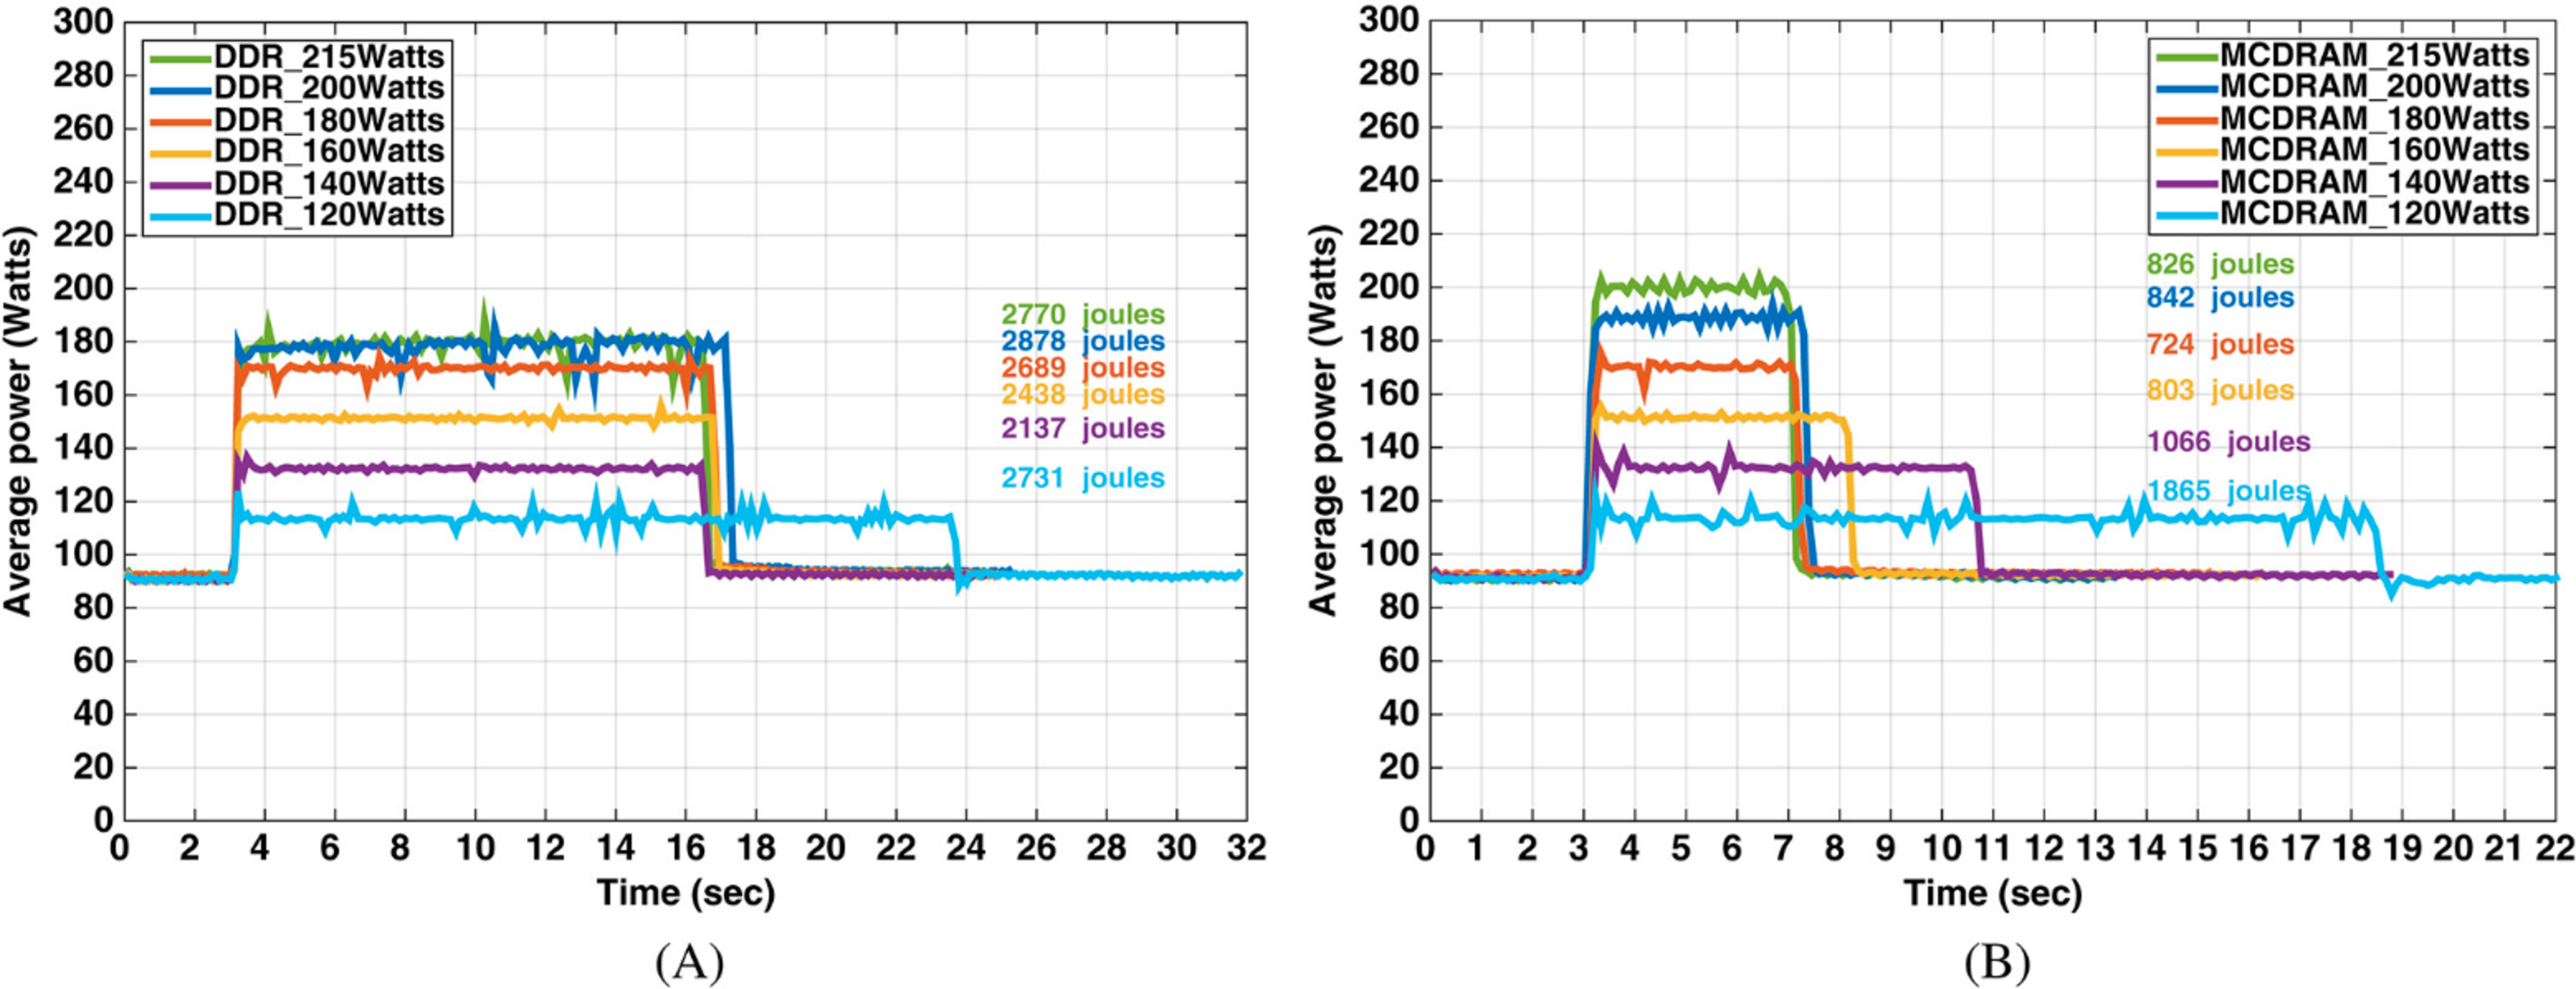
\includegraphics[width=0.82\textwidth]{projects/2.3.2-Tools/2.3.2.06-EXA-PAPI/Exa-PAPI-jacobi.pdf}
\caption{Average power measurements (Watts on y axis) of Jacobi algorithm on a 
12,800 x 12,800 grid for different power caps. (A) FLAT mode: data allocated to DDR4; 
(B) FLAT mode: data allocated to MCDRAM}
\label{fig:Jacobi_power}
\end{center}
\end{figure}
%
\vspace{-8pt}

On the software-defined events front, we have already proposed an API
(publicly available on Jira:
\url{https://jira.exascaleproject.org/secure/attachment/12251/2017_SDE_API_report.pdf})
and received significant feedback and requests for changes by members of the
runtime and library communities, which we have incorporated. We have also
developed a prototype implementation of an SDE component in PAPI, which we are
using to integrate SDE support in various ECP projects, such as:
%
\begin{enumerate}
\vspace{-3pt}
\item ByFL (HT-DSE): \url{https://bitbucket.org/jagode/byfl_papi_sde}
\vspace{-5pt}
\item PaRSEC (2.3.1.09 STPM11-ParSEC): \url{https://bitbucket.org/herault/parsec/branch/PAPI-SDE}
\vspace{-5pt}
\item PEEKS (2.3.3.10 STMS11-PEEKS): \url{https://bitbucket.org/icl/magma} (branch: \verb+PAPI_SDE+)
\vspace{-5pt}
\item NWchemEx (2.2.1.02 ADSE11-NWChemEx): \url{https://bitbucket.org/jagode/nwchem_papi_sde}
\end{enumerate}

\paragraph{Next Steps}

Our next efforts will focus on:
\begin{enumerate}
\item \textbf{Development of a PAPI component for IBM Power9 Hardware Counter
	Support:} Add support for (1) core performance events, which are specific
		to each core; and (2) shared events, which monitor the performance of
		node-wide resources that are shared between cores. Access to shared
		events require elevated privileges. However, IBM's official route for providing
		access to shared events will be through the
		Performance Co-Pilot (PCP) for non-root users. Thus, one of the
		Exa-PAPI efforts is to develop a PAPI-PCP component so that all users
		can access Power9 shared events through PAPI.
%
\item \textbf{Release of PAPI's SDE component, and integration of SDEs with other ECP efforts}: 
		Refine the PAPI SDE prototype implementation based on
		feedback from the ECP community and experience acquired from
		instrumenting ECP projects. Instrument ECP libraries, runtimes, and
		applications, such as PaRSEC, PEEKS, and NWChem to use software-defined
		events to export performance information.
\end{enumerate}
